 \chapter{Requirements and Analysis}

With the introduction to Manta Flow platform covered, we now have enough information required to understand and analyze the problem of embedded code analysis in its context. In this chapter we will first present a motivational example for embedded code analysis, discuss requirements set by Manta Flow stakeholders, analyze multiple data technologies that support embedded code and finally we will analyze how to integrate embedded code analysis into scanners.

\section{Purpose of embedded code analysis}

We have already briefly explained what embedded code is and why it makes sense to analyze it in Manta Flow. Let us present an example that will support this explanation. It can help us build a better understanding of the motivation and illustrate some of the challenges that we need to overcome.
\par
This example is based on a real customer inquiry. A company has decided to move a part of their systems from self-hosted solution to a cloud-based solution. The migrated system cleans, pre-processes and combines data from multiple sources to create a high-quality data source for business analyses. They decided to use AWS (Amazon Web Services) as their cloud service provider. The new pipeline uses Amazon S3, Amazon Redshift and AWS Glue. Amazon S3 is a cloud object storage which is often used to store files used by other services. Amazon Redshift is a data warehousing service based on PostgreSQL database and optimized for scalability and big data processing. AWS Glue is an ETL tool which we have already introduced and will work with later in the thesis. The transformation jobs in AWS Glue are written in Python. The pipeline roughly follows these steps~(shown in Figure~\ref{fig:pipelineExample}):
\begin{enumerate}
    \item Files containing raw unprocessed data are uploaded to Amazon S3.
    \item An AWS Glue job is executed which reads these files and normalizes the data - fills empty values, normalizes column names, etc. and stores it in a common data format under curated files on Amazon S3.
    \item Other AWS Glue jobs can be executed which read one or several curated files, combine the data and store it in a table in Amazon Redshift.
    \item Amazon Redshift is the final destination of this data pipeline. It is then used as a data source for visualisations and analytics.
\end{enumerate}

\begin{figure}[ht]\centering
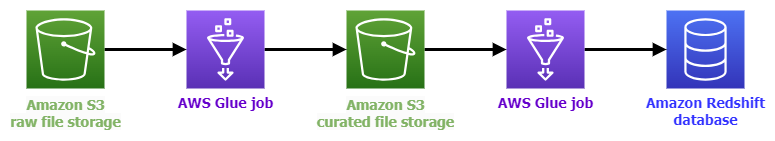
\includegraphics[width=1.0\textwidth]{img/pipeline_example.png}
\caption{A diagram of data flows in the pipeline}
\label{fig:pipelineExample}
\end{figure}

\par
Projects of this magnitude may take several months to complete, involve tens of employees who spend hundreds to thousands of man-days working on it. At this scale, it is important to keep a good overview on the progress to complete the project successfully. The customer has previously used Manta Flow to analyze different systems and would like to use it on this project as well. They would like to use it initially to watch the migration process and ensure that the new pipeline behaves correctly and no processes have been missed. After the project is over, they would like to continue using it to help with maintenance and problem resolution. The final dataset is a source for important financial and customer behavior analyses which directly impact many business decisions, so it is critical that the data is assembled correctly and data lineage visualization can help in that effort.
\par
How can data lineage analysis of embedded code help the customer? The pipeline consists of two data storage technologies, Amazon S3 and Amazon Redshift. They are only locations where data is stored. In order to find out how, for example, values in column \textit{average\_price} in table \textit{Sales} are computed, we must look into one of the AWS Glue jobs. An AWS Glue job runs a Python or Scala script on Apache Spark engine, which is a popular engine for large-scale data analytics. Therefore to provide the data lineage graph, we must run data flow analysis of the job's embedded code. When the analysis is successful, to find out how a value is computed we simply need to click on it in the visualized graph and follow the lineage. Without it we would have to locate the job manually, which might not be easy among 10s or 100s of them.

%%%%%% TODO
% 1 vziat requirements a rozpisat ich ako poziadavky zo strany Manty, zanalyzovat a vysvetlit ich
% 2 rozsirit analyzu technologii, pridat nejake priklady. 
% 3 Nasleduje analyza, ze to bude nejaka service atd, kde priblizime, ako funguje query service a porovnanie, co je stejne, co je odlisne a co by slo vyuzit
% Na konci kapitoly musi byt jasne, co ideme robit

\section{Requirements from Manta}

As this work has been assigned by and developed in cooperation with Manta Tools company which develops Manta Flow, they have set certain requirements that the final solution should fulfill. In this section we will first, state a requirement and then we will follow-up with a discussion about its motivation and implications. We will also use a new term \textit{source technology}. In the context of embedded code analysis, the source technology is the data technology that uses embedded code. In the previous example, the source technology is AWS Glue which uses Python embedded code.

\subsection{Functional requirements}

These requirements define what the solution needs to and needs not to do.

\subsubsection{Embedded code analysis}

\textit{Provided a code script (string/file, not important implementation detail) and configuration, the service analyzes the script and delivers lineage graph for that script}. This requirement is pretty straight-forward, it describes what is to be delivered.
\par
Firstly, we shall discuss why a service is required. \textit{Service} is a wide term and its concrete meaning depends on the context. There is already \textit{Dataflow Query Service} in Manta Flow which handles analysis of embedded database queries and scripts. In its core it is a Java bean (a class that encapsulates one or more objects into a single standardized object) which uses specific parts of database scanners to process the queries. It is called a service, because it is a reusable component (a bean) that can be used by any scanner and it provides its services through a standardized interface with a specific input and output. The solution described in this work, Embedded Code Service, is in many ways similar to Dataflow Query Service so it is expected to be used in a similar way.
\par
The service shall accept embedded code as one of its inputs. That is different from how scanners in Manta Flow usually work, because they collect their inputs themselves. It shall also accept configuration. What will it be used for? Scanners in Manta Flow have many configurable properties which influence their execution, users may modify them in \textit{Manta Admin UI}. It must be possible to configure how embedded code is analyzed as well. Additionally, from the description of embedded code we know that it is executed in the environment provided by the data technology. This environment can differ from standard runtime environment, so any differences, e.g. environment variables, pre-included libraries, need to be passed to the service in some way - in the configuration.
\par
The last part of this requirement describes that the service shall perform data flow analysis of the input and provide the data lineage graph on the output for further processing. Contrary to the standard scanner workflow, the Manta graph is not uploaded to \textit{Manta Flow Server}, but returned as return value.

\subsubsection{Graph merging}

\textit{The service can merge the lineage graph with the lineage graph of parent data technology when provided a node to be merged with}. This requirement extends the previous one and describes what is to be done with the output.
\par
Each scanner produces one Manta graph for one input. When it uses a service to process a part of the input, which creates other graphs, they need to be merged. Furthermore, edges can be created only between nodes present in the graph, so if there is a data flow between the objects in the source technology graph and objects in embedded code graph, they need to be merged into one so that the edge representing the data flow can be added. The merge operation is not a trivial process, so it shall be the responsibility of the service to implement it. The benefits are easy to see, no need to implement it each time the service is used across different scanners, which improves maintainability of the solution and also there is no need to understand it outside of the service. The developers may simply use the service interface to merge the results.

\subsubsection{Multi-purpose service}

\textit{The service can support multiple parent data technologies - technologies that support usage of user-defined embedded code}. This requirement states that the service is multi-purpose, so there is one such service available instead of there being many services for processing embedded code in each data technology.

\subsection{Qualitative (non-functional) requirements}

On top of the definition of functionality of the solution, there are also some requirements defining its qualities.

\subsubsection{Optimized for scanning}

\textit{The service should be optimized to handle tens to hundreds of scripts for a specific combination of technology-scanner in one analysis - the limitation should be the speed of the scanner, not the speed of the service}. In general, the service can be expected to be used multiple times by one scanner when it processes one connection, there may be several embedded code scripts. It is important to keep that in mind in its design. The service is intended to facilitate data lineage scanning and most of its execution time should be spent doing so. All other work that the service needs to do shall be reasonably optimized so that this overhead does not add up to a lot when it is called multiple times. This requirement does not intend to include specific scanner optimizations that can be made to improve the overall execution time of the service as they shall be evaluated after this solution is implemented and are outside of the scope of this work.

\subsubsection{Extendibility}

\textit{Extending supported data technologies should be simple, adding a new technology should only include collecting its configuration in the technology scanner and implementing this configuration in Embedded Code Service}. It is expected that the list of the scanners that use the service will grow in time based on customer requirements and available development capacity. The service shall be designed in a way that promotes extendibility so that the effort required to add support for new data technology is minimised. This can be done by splitting the code base to a common and a specific part so that it is obvious what needs to be added or modified in order to extend the service.

\subsubsection{Code reuse}

\textit{Maximize code reuse. Reuse the existing scanners and logic}. Scanners for analyzing programming language source code are very complex. We shall use the existing scanners and make only the necessary modifications to be able to analyze embedded code. Developing one scanner for analyzing both applications and embedded code is a preferred way from resource allocation perspective.

\subsubsection{Code duplication}

\textit{Minimize code duplication, no logic should be written on more than one place}. One of the purposes of the service is to hide repeating blocks of code that are tied with its use. Deduplication improves maintainability, because when a process needs to be changed, it only needs to be changed in one place instead of in multiple location. One of the examples of such practice is graph merging logic mention in one of the previous requirements.

%%----- SECTION -----%%
\section{Source technology analysis}

Before we dive further into the analysis, we need to examine which source data technologies, whether currently supported by Manta Flow or planned, support embedded code. Limiting to these technologies is driven by business requirements, it does not make sense to support analysis of embedded code in a data technology that is not used by any current or prospective customer. This overview will give us a better understanding of the range of embedded code use-cases, their similarities and differences.

\subsubsection{Hive}
Hive is a distributed data warehouse system that allows users to read, write and manage big volumes of data using SQL. Starting from version 0.13.0, it supports writing user-defined functions in Java which accept parameters and return a value. The function is implemented by a class that extends a Hive \texttt{UDF} base class. These base classes define methods that shall be implemented by the function and will be invoked in specific order on SQL query execution. This class is then supposed to be packaged in a JAR referenced by a URI from which it will be loaded into the environment~\cite{hive}. An example of a user-defined function implementation that turns a string into lower case can be seen in Figure~\ref{fig:hiveScript}.

\begin{figure}[ht]
\begin{lstlisting}[language=Java]
package com.microsoft.examples;

import org.apache.hadoop.hive.ql.exec.Description;
import org.apache.hadoop.hive.ql.exec.UDF;
import org.apache.hadoop.io.*;

// Description of the UDF
@Description(
    name="ExampleUDF",
    value="returns a lower case version of the input string.",
    extended="select ExampleUDF(deviceplatform) from hivesampletable limit 10;"
)
public class ExampleUDF extends UDF {
    // Accept a string input
    public String evaluate(String input) {
        // If the value is null, return a null
        if(input == null)
            return null;
        // Lowercase the input string and return it
        return input.toLowerCase();
    }
}
\end{lstlisting}
\caption{An example of a Hive user-defined function written in Java~\cite{hiveudfexample}}
\label{fig:hiveScript}
\end{figure}

\subsubsection{Microsoft SQL Server}
Microsoft SQL Server enables users to implement stored procedures, triggers, user-defined types, user-defined functions (scalar and table valued), and user-defined aggregate functions using any .NET Framework language, including Microsoft Visual Basic .NET and Microsoft Visual C\#. They can be implemented by arbitrary classes and methods as long as they are properly annotated. These annotations facilitate the lookup and binding between SQL Server and embedded code. Compiled code is distributed in DLL and loaded into environment using SQL syntax~\cite{mssql}.

\subsubsection{SQL Server Integration Services (SSIS)}
SSIS is a platform for data integration and transformation solutions. It provides graphical tools for building ETL workflows, but it is also possible to create custom objects programmatically in C\# or Visual Basic. These include tasks, connection managers, log providers, enumerators and data flow components. Implementations of custom objects are expected to extend one of the base classes provided by SSIS, to override required methods and to use proper attributes. These objects are then distributed as a compiled class library. This is a similar approach as that of MSSQL~\cite{ssis}.

\begin{figure}[ht]
\begin{lstlisting}[language=csh]
using System;
using System.Data;
using Microsoft.SqlServer.Dts.Pipeline.Wrapper;
using Microsoft.SqlServer.Dts.Runtime.Wrapper;

[Microsoft.SqlServer.Dts.Pipeline.SSISScriptComponentEntryPointAttribute]
public class ScriptMain : UserComponent
{
    public override void CreateNewOutputRows()
    {
        // Accessing input column values
        string inputColumnValue = string.Empty;
        if (Variables.MyInputColumn != null && Variables.MyInputColumn.Length > 0)
        {
            inputColumnValue = Variables.MyInputColumn[0].ToString();
        }

        // Performing some transformation on the input column value
        string outputColumnValue = inputColumnValue.ToUpper();

        // Creating new output rows
        Output0Buffer.AddRow();
        Output0Buffer.MyOutputColumn = outputColumnValue;
    }
}
\end{lstlisting}
\caption{An example of an SSIS script component written in C\#}
\label{fig:cSharpScript}
\end{figure}

\par
In an example shown in Figure~\ref{fig:cSharpScript}, a script component is defined as a class which inherits from the \texttt{UserComponent} base class provided by SSIS. The \texttt{CreateNewOutputRows} method is overridden to implement the desired logic. Within it we can access the input column values using the \texttt{Variables} object, which provides access to the input columns. In this example, the value of the first input column (\texttt{MyInputColumn}) is retrieved and stored in the \texttt{inputColumnValue} variable. Next, a transformation is performed on the input column value (in this case, converting it to uppercase), and the result is stored in the \texttt{outputColumnValue} variable. Finally, a new output row is added using the \texttt{OutputBuffer} object, and the transformed value is assigned to the output column (\texttt{MyOutputColumn}).

\subsubsection{Snowflake}
Snowflake Data Cloud is a cloud-based data storage and analytics service. It is common to use SQL to interact with data in Snowflake and embedded code is integrated in a similar way in the form of functions and stored procedures. Apart from SQL, these can be written in multiple programming languages - Java, Scala, JavaScript or Python. Each language used has (slightly) different capabilities and requirements. In case of JavaScript, it can be used to execute SQL statements and interact with the result to provide a return value. Java, Scala and Python scripts have to contain a function or a method with the first argument of type \texttt{Session} from Snowflake's Snowpark library. This argument will be populated by Snowflake when the procedure/function is invoked and is used for interaction with Snowflake platform~\cite{snowflake}.

\begin{figure}[ht]
\begin{lstlisting}[language=SQL]
CREATE OR REPLACE PROCEDURE my_stored_procedure(param1 STRING, param2 INT)
RETURNS STRING
LANGUAGE PYTHON
AS
$$
    import snowpark as sp

    @sp.session
    def my_snowpark_function(session):
        # Create a DataFrame using the provided parameters
        df = session.range(0, param2).select(sp.lit(param1).alias('Value'))
        
        # Perform some transformations on the DataFrame
        transformed_df = df.withColumn('Length', sp.length(df['Value']))
        
        # Convert the transformed DataFrame to a Pandas DataFrame
        pandas_df = transformed_df.toPandas()
        
        # Generate a summary string
        summary = pandas_df.describe().to_string()
        
        return summary
    
    # Call the Snowpark function with the provided parameters
    return my_snowpark_function(param1, param2)
$$;
\end{lstlisting}
\caption{An example of a Snowflake stored procedure written in Python}
\label{fig:snowflakeScript}
\end{figure}

\par
In an example shown in Figure~\ref{fig:snowflakeScript}, we are creating a stored procedure written in Python that takes two parameters, a string and an integer. The body of the stored procedure contains a Python function named \texttt{my\_snowpark\_function}. This function uses the Snowpark session decorator to establish a session with Snowflake. Within the function, we create a DataFrame and perform some transformations on it. In this example, we add a new column \textit{Length} that calculates the length of the \textit{Value} column. Next, we convert the transformed DataFrame to a Pandas DataFrame and generate a summary string from it. Finally, the stored procedure calls the \texttt{my\_snowpark\_function} with the provided parameters and returns the summary string.

\subsubsection{Databricks}
Databricks is a web-based data platform that combines data warehouses and data lakes with analytics build on Apache Spark and IPython-style notebooks. These notebooks are interactive computational environments. They consist of a sequential combination of cells which may contain rich text, embedded code, data visualization etc. Embedded code cells may be written in Python, Scala, SQL or R and it is possible to combine cells written in different languages in one notebook. During a notebook execution, cells written in the same language are executed in the same environment and may interact with other language environments using shared context of Apache Spark~\cite{databricks}.
\par
Let us have a notebook consisting of a Python cell (shown if Figure~\ref{fig:pythonDatabricks}) and an SQL cell (shown in Figure~\ref{fig:sqlDatabricks}). The Python cell sets the value of the shared variable which is then printed to the standard output. The SQL cell showcases how to access the shared variable within an SQL statement using the \$ symbol. In this example, we update the value of column1 based on the value stored in the shared variable.

\begin{figure}[ht]
\begin{lstlisting}[language=Python]
# Define a shared variable
dbutils.shared.notebook.set("my_shared_variable", "Hello, Databricks!")

# Access the shared variable
shared_value = dbutils.shared.notebook.get("my_shared_variable")
print(shared_value)
\end{lstlisting}
\caption{Python cell of a Databricks notebook}
\label{fig:pythonDatabricks}
\end{figure}

\begin{figure}[ht]
\begin{lstlisting}[language=SQL]
-- Update a table using the shared variable in SQL
UPDATE my_table
SET column1 = $my_shared_variable
WHERE condition;
\end{lstlisting}
\caption{SQL cell of a Databricks notebook}
\label{fig:sqlDatabricks}
\end{figure}

\subsubsection{AWS Glue}
AWS Glue is a fully managed ETL service provided by Amazon Web Services (AWS). It simplifies the process of preparing and loading data for analytics, data warehousing, and other data-related tasks. With AWS Glue, you can create and schedule ETL jobs to automate the data transformation and loading process. It handles the execution, monitoring and orchestration of these jobs. ETL jobs leverage the underlying Apache Spark framework for distributed data processing. Each job is defined by a script written in Python or Scala. This script can be written manually or the job's workflow is built in an interactive GUI and the code is generated automatically. Compared to other data technologies, AWS Glue is built entirely on embedded code. That means that each ETL job is executed entirely by a single Python/Scala script as opposed to only parts of data operations in other data technologies~\cite{awsglueintro}.
\par
The example in Figure~\ref{fig:embeddedScript} show code of an ETL job that performs data processing and transformation, combining data from different sources and storing the result in an S3 bucket. Firstly, we read data from a specified database and tables into dynamic frames on which we perform data transformations. The \texttt{products} frame is modified by dropping certain fields and renaming one. Multiple joins are applied to the frames, first between \texttt{products} and \texttt{purchases}, and then between the resulting frame and \texttt{suppliers}. The resulting frame is written to an S3 location in the parquet format.

\begin{figure}[ht]
\begin{lstlisting}[language=Python]
import sys
from awsglue.transforms import Join
from pyspark.context import SparkContext
from awsglue.context import GlueContext

glueContext = GlueContext(SparkContext.getOrCreate())

db_name = "main_db"
output_dir = "s3://glue-example/output/supply_chain"

# Create dynamic frames
products = glueContext.create_dynamic_frame.from_catalog(database=db_name, table_name="products_json")
purchases = glueContext.create_dynamic_frame.from_catalog(database=db_name, table_name="purchases_json")
suppliers = glueContext.create_dynamic_frame.from_catalog(database=db_name, table_name="suppliers_json")

# Keep the fields we need and rename some
products = products.drop_fields(['color', 'identification']).rename_field('name', 'product_name')

# Join the frames
result = Join.apply(Join.apply(products, purchases, 'id_product', 'product_id'), suppliers, 'supplier_id', 'id_supplier')

# Write out the frame into parquet file
glueContext.write_dynamic_frame.from_options(frame = result, connection_type = "s3", connection_options = {"path": output_dir}, format = "parquet")
\end{lstlisting}
\caption{An example of an embedded script in AWS Glue}
\label{fig:embeddedScript}
\end{figure}

\subsubsection{PostgreSQL}
By default, PostgreSQL supports functions written in C, but theoretically users may use any language, as long as it can be made compatible with C, e.g. C++. However, that is often difficult due to different calling conventions, so its safe to assume C language is used. The function definitions are supposed to use macros from \texttt{postgres.h} header file, but otherwise are common C functions. The code is compiled and dynamically loaded into the environment using SQL. There is currently no plan to support analyzing C language, so this data technology is mentioned only for completeness and to illustrate that there are also other ways~\cite{postgresql}.

\subsubsection{Other data technologies}
Besides the data technologies already described, there are others that provide embedded code integration and are supported in Manta Flow. These follow similar principles as some that were already described before, so we will not cover them in detail. However, we list them below for completeness:
\begin{itemize}
    \item Talend supports extending the functionalities of a Talend Job using custom Java commands~\cite{talend}.
    \item Google BigQuery supports defining functions written in JavaScript~\cite{bigquery}.
    \item StreamSets allows creating custom StreamSets processors in Java~\cite{streamsets}.
    \item Informatica supports creating custom components with Java~\cite{informatica}.
    \item Azure Data Factory supports creating Custom activity with own data movement or transformation logic in C\# that can be added to a pipeline~\cite{adf}.
    \item SAS supports running Python statements within a SAS session~\cite{sas}. Additionally, there are multiple Python packages for interacting with SAS from Python.
\end{itemize}

\subsection{Embedded code usage philosophy}
Based on the description of embedded code usages, we can observe a few repeating patterns. These will help us design Embedded Code Service.
\par
We can see that database systems use embedded code in the form of user-defined functions or stored procedures. They can then be invoked as a part of an SQL query or an SQL script. They often return a value and may receive arguments.
\par
Another common use-case is to define a custom transformation or a task in an ETL workflow. The details of this use-case vary more than those in database systems but in general they implement a specific interface which functions are invoked in a pre-determined order by the data technology.
\par
Next observation relies to the programming language being used. Most often we can see Java or Scala, .NET languages (mainly C\# or Visual Basic) and Python. Sometimes also JavaScript is used and there is one case of R and C, but we shall ignore them as there isn't currently a language scanner implemented in Manta Flow for them.
\par
In compiled static-typed languages (Java and C\#), it is common to tag the classes that shall be used as embedded code and require a rigid interface, either by extending a base class or using annotations. The code is distributed in compiled form and loaded dynamically. Interaction with the data technology is facilitated through an object that is provided as a method argument or a property of a base class.
\par
As Python is interpreted and not compiled, it is possible to inject the embedded code into a different code to create a new script. That allows use-cases where some code is executed before embedded code which defines some variables, functions, classes etc. The embedded code may then directly read these identifiers without having to declare them, which is used to provide interface for interacting with data technology. To successfully analyze such approach, it is important to understand and simulate these assignments.

%%----- SECTION -----%% 
\section{Embedded Code Service analysis}

Based on the requirements set by Manta Tools and the analysis of data technologies that use embedded code, we are going to focus on the analysis of problems related to the implementation of Embedded Code Service in a more specific manner in this chapter.
\par
Let us first summarize what we have learned so far. Embedded Code Service is responsible for analyzing data lineage in code embedded in various data technologies and merging its lineage graph to that of the source technology. Similarly to Dataflow Query Service, it enables merging of data lineage of two cooperating technologies into one graph utilizing the existence of separate scanners for each of the respective technologies. It provides a way to compose a more complete lineage for the given technology without the need to implement the specifics of analyzing the embedded code within the source technology scanner.
\par
We have mentioned the similarity to Dataflow Query Service so many times that we finally need to explain why analysis of embedded code is not handled by it. They both analyze some form of embedded scripts. It would be possible to modify it for such use-case, but it would not be practical for several reasons.
\par
Firstly, the scenarios when they are used are different. Dataflow Query Service is used to analyze queries without requiring much information about them. When a query is used outside of a database, it is not always easy to detect what kind of database is being queried. Dataflow Query Service polls every scanner to decide if it can process the query and lets the first one that answers positively to do so, so this logic does not need to be implemented each time the service is used. When analyzing embedded code, this information is always known so there is no need for such process.
\par
Secondly, the interfaces of the services do not overlap. To analyze a script, Dataflow Query Service requires connection details whereas Embedded Code Service requires a configuration object. Furthermore, interface of Dataflow Query Service contains a lot of methods used to deduce database objects. That is not needed or wanted in case of embedded code.
\par
Due to these two reasons a decision was made to create a new service for the analysis of embedded code. Having only one would not be practical and would not bring any reasonable benefits. However, that does not mean that they have to be completely different. There are a few great solution in Dataflow Query Service that we can use so that we do not reinvent the wheel. There are quite a few more problems that we need to address before we can move on with design and implementation. Here is the list for an overview:
\begin{enumerate}
    \item Merging embedded code graph to the enclosing technology graph
    \item Specifying runtime configuration - available libraries etc.
    \item Caching
\end{enumerate}
Let us now take a closer look at each of them.

%%-subsection-%% 
\subsection{Merging embedded code graph with the source technology graph}
The graphs contain a set of nodes and a set of edges between them. When two graphs are merged, the easy part is copying the nodes and edges from one graph to the other. Sometimes, embedded code uses data or data source originating from the pipeline in the source technology. We have already shown that in SSIS example in Figure~\ref{fig:cSharpScript}. In the example code, the function reads the input dataset and writes data to the output dataset. To create a complete lineage, when merging two graphs we also need to correctly map the equivalent nodes present in the embedded code graph to those of the source technology graph. This is the difficult part of merging two graphs.
\par
The problem is that there is not always enough information in embedded code to resolve the input or the output. In the example, the exact structure or origin of the input dataset is not known, we only know that it contains a\texttt{MyInputColumn} column. Similarly, we only know that the output dataset has a \texttt{MyOutputColumn} column. We can easily create the column nodes from this information and connect them with an edge respecting the data flow, but the column nodes cannot exist on their own, they need to be assigned a parent node that represents the dataset. A naive solution would be to add specific nodes representing input and output datasets of SSIS script transformation and assign them as the parents of column nodes. In source technology we could locate such nodes in embedded code graph and merge them with their equivalent (essentially, moving all edges from old node to the new node by changing edge starting or ending points). This approach would work, but is too specific. The programming language scanner needs to create specific nodes for each source technology endpoint, each source technology has to locate specific nodes and with each extension a lot of new code has to be added into both scanners. We would prefer a more generic approach.
\par
Dataflow Query Service introduces a concept of \textit{pin nodes} which is described in section~\ref{section:DQS}. This concept is well-suited to be also used in our service, although with a couple of modifications. All nodes created in a query are a part of the query so pin nodes serve only as external connection points which may or may not be used. In embedded code, we would like to use them as placeholders for nodes we do not know but we know they exist, so we can connect an edge to them. These nodes could be created by a programming language scanner when it processes a data flow with unknown origin. This would alleviate the struggle to create a new type of node for a new source technology endpoint, because a generic pin node will be created each time. We have to make sure we do not create two identical pin nodes for different connection points. Pin nodes can be distinguished by their name (each node in a graph must have a name) and they only exist until the embedded code graph is merged, so they only need to be unique while embedded code is analyzed which can easily be checked by the scanner.
\par
We have solved creation of data flows between nodes with unknown origin in embedded code, but we still need to find out how we can connect source technology graph to correct pin nodes. A naive solution could encode pin node details into its name, for example \texttt{SSIS\_PIN\_NODE\_SCRIPT\_COMPONENT\_INPUT\_DATASET\_MyInputColumn\_COLUMN}. A source technology could enumerate all pin nodes that need to be mapped, decode their names and connect them with their equivalents. This is a feasible solution, but it lacks a bit of finesse, because serializing and deserializing information into strings is a tedious process.
\begin{figure}[ht]\centering
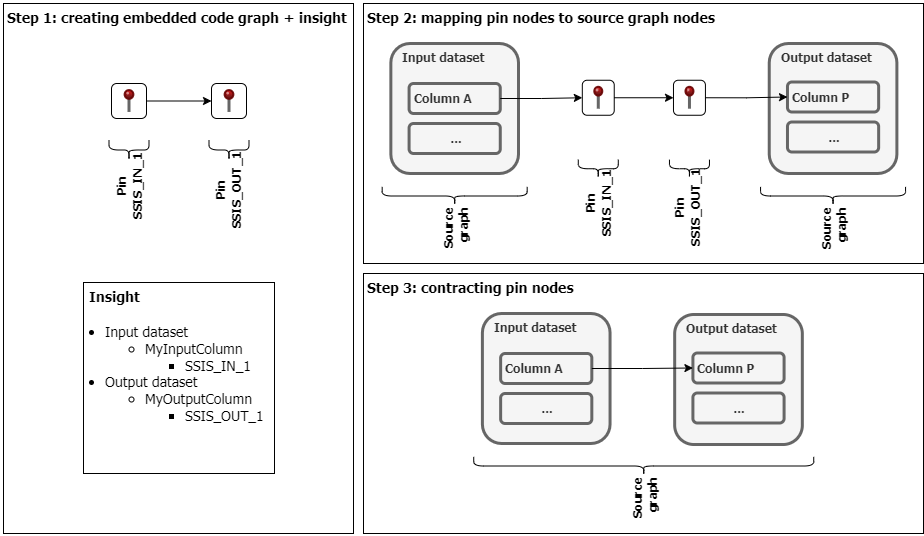
\includegraphics[width=1.0\textwidth]{img/pin_nodes_ecs.png}
\caption{A diagram of the pin node mapping process in Embedded Code Service}
\label{fig:pinNodesECS}
\end{figure} 
\par
What if instead we could pass some information about the input to a programming language scanner and also retrieve some information from its execution after it ends? Such mechanism would help create a more precise graph for embedded code, because it would provide the scanner with a better contextual information, but it would also allow us to pass information about the created pin nodes without having to serialize it in their names. This mechanism requires changes to be made in programming language scanners which we would like to avoid if we can, but it turns out that such mechanism can bring great benefits. The mechanism is called \textit{Insight and Outsight} and was developed by other developers outside of the scope of this thesis. We shall describe it in more detail later when we discuss design and implementation. For now we only need to know that the information about created pin nodes is passed to the source technology in an \textit{Insight} which is used to easily map them.
\par
The mapping process is depicted in Figure~\ref{fig:pinNodesECS}. Code shown in Figure~\ref{fig:cSharpScript} was used for this diahram. It shows how the embedded code graph would look like when pin nodes are involved, how they are mapped using an \textit{Insight} and the result after contracting pin nodes.

%%-subsection-%% 
\subsection{Specifying runtime configuration}
When embedded code is executed in source technology, the technology prepares the runtime environment in which it executes the code. This environment can often be configured by the user at which point it is necessary to propagate this information to the scanner. More importantly, some data technologies allow specifying other libraries to be included at runtime (AWS Glue, Databricks). The embedded code does not contain these libraries, they are managed by the source technology, but they can be imported and used which requires them to be included in the analysis. It means that Extractor for source technology needs to extract these libraries and they need to be provided to Embedded Code Service in configuration as well as values of configurable properties.
\par
Currently, programming language scanners are expecting that all analyzed code is present in one directory after the extraction. Because there may be additional files included in configuration that need to be analyzed, the service needs to perform \textit{input orchestration}. The goal of input orchestration is to organize the files in input directory as they would be organized in runtime environment of source technology. Extractor of the programming language scanner can then use the input orchestrated in this way to produce an input for Reader. When orchestrated successfully, Reader would not be able to recognize any difference and would be able to analyze the code correctly.
\par
In general, it is difficult to estimate what properties need to be passed about runtime configuration for all technologies and languages. Furthermore, it is also not possible to to perform the orchestration in a general way due to the differences of each source technology. However, we don’t need to specify that in a general way. This information is only relevant for the source technology which needs to prepare the configuration, because it knows what can and needs to be provided. Embedded Code Service does not need to know the details outside input orchestration, which will be different for each data technology. Therefore, the configuration contract only needs to exist between source technology and input orchestration component, so it can be highly customizable. Using polymorphism for runtime configuration seems like a good choice as it can provide both a type-safe and customizable interface.

%%-subsection-%% 
\subsection{Caching}
It is also necessary to address the possibility of caching some intermediate data. It can be expected that multiple instances of embedded code can appear during one analysis (multiple scripts within source technology analysis). These instances have a lot in common. Since they are embedded, they rely on some part of the environment to be provided by the source technology and this part is often the same. It is therefore valid to consider if some analysis parts can only be computed once and then cached and reused to improve performance. 
\par
Sadly, we were not able to find a universal answer and solution that can be implemented by Embedded Code Service. There can be some small opportunities in particular cases but we have not found a general solutions. However, these particular cases should be reviewed for each programming language scanner to see whether they can bring valuable performance benefits.
\par
First opportunity is during input orchestration. As we mentioned earlier, part of the runtime is often the same, so when it is generated and prepared for the first time, it can be stored so it does not need to be generated again. It can be beneficial if this common runtime is considerably large compared to the size of embedded code and the duration of the analysis. For example, currently in Python scanner, parsing standard library which consists of ~2000 files takes longer than performing the analysis of a short script (<100 LOC). In a situation when there are tens or hundreds of such scripts, the improvement could save customer a lot of time. The standard library is available for each script, therefore it could be parsed once and reused. On the other hand, for Bytecode and C\# the input needs to be compiled, so each entry point has to be prepared individually.
\par
The other reviewed opportunity is during the analysis. Since we often use the same dependencies, we could cache some intermediate results when analyzing flows in them. However, this optimization is already implemented within the scanners themselves. They use plugins for libraries that mimic the propagation of data flows in library functions and methods, so essentially, no library code is analyzed. Additionally, the execution of the worklist algorithm used for static analysis of the code is highly dependent on the inputs, so it behaves differently for each entry point and therefore there are no shared data between two entry points.
\par
In conclusion, when implementing a new combination of technology-language in Embedded Code Service, it is advised to review the possibility of caching a part of input preparation as it can influence the overall performance of the source technology scanner. This recommendation will be a part of guidelines for implementing input orchestration for a new source technology.